\section{Auswertung}
\label{sec:Auswertung}

\subsection{Schwellenstrom}
\label{Schwelle}
Bei einem Schwellenstrom von $\SI{34,5}{\milli\ampere}$ tritt Lasergranulation auf. In \autoref{fig:granulation}
sind die entsprechenden Bilder der Lasergranulation zu finden. Über dem Schwellenstrom ist außerdem ein starkes
Ansteigen der Intensität zu beobachten.

\begin{figure}
    \begin{subfigure}[c]{0.5\textwidth}
        \centering
        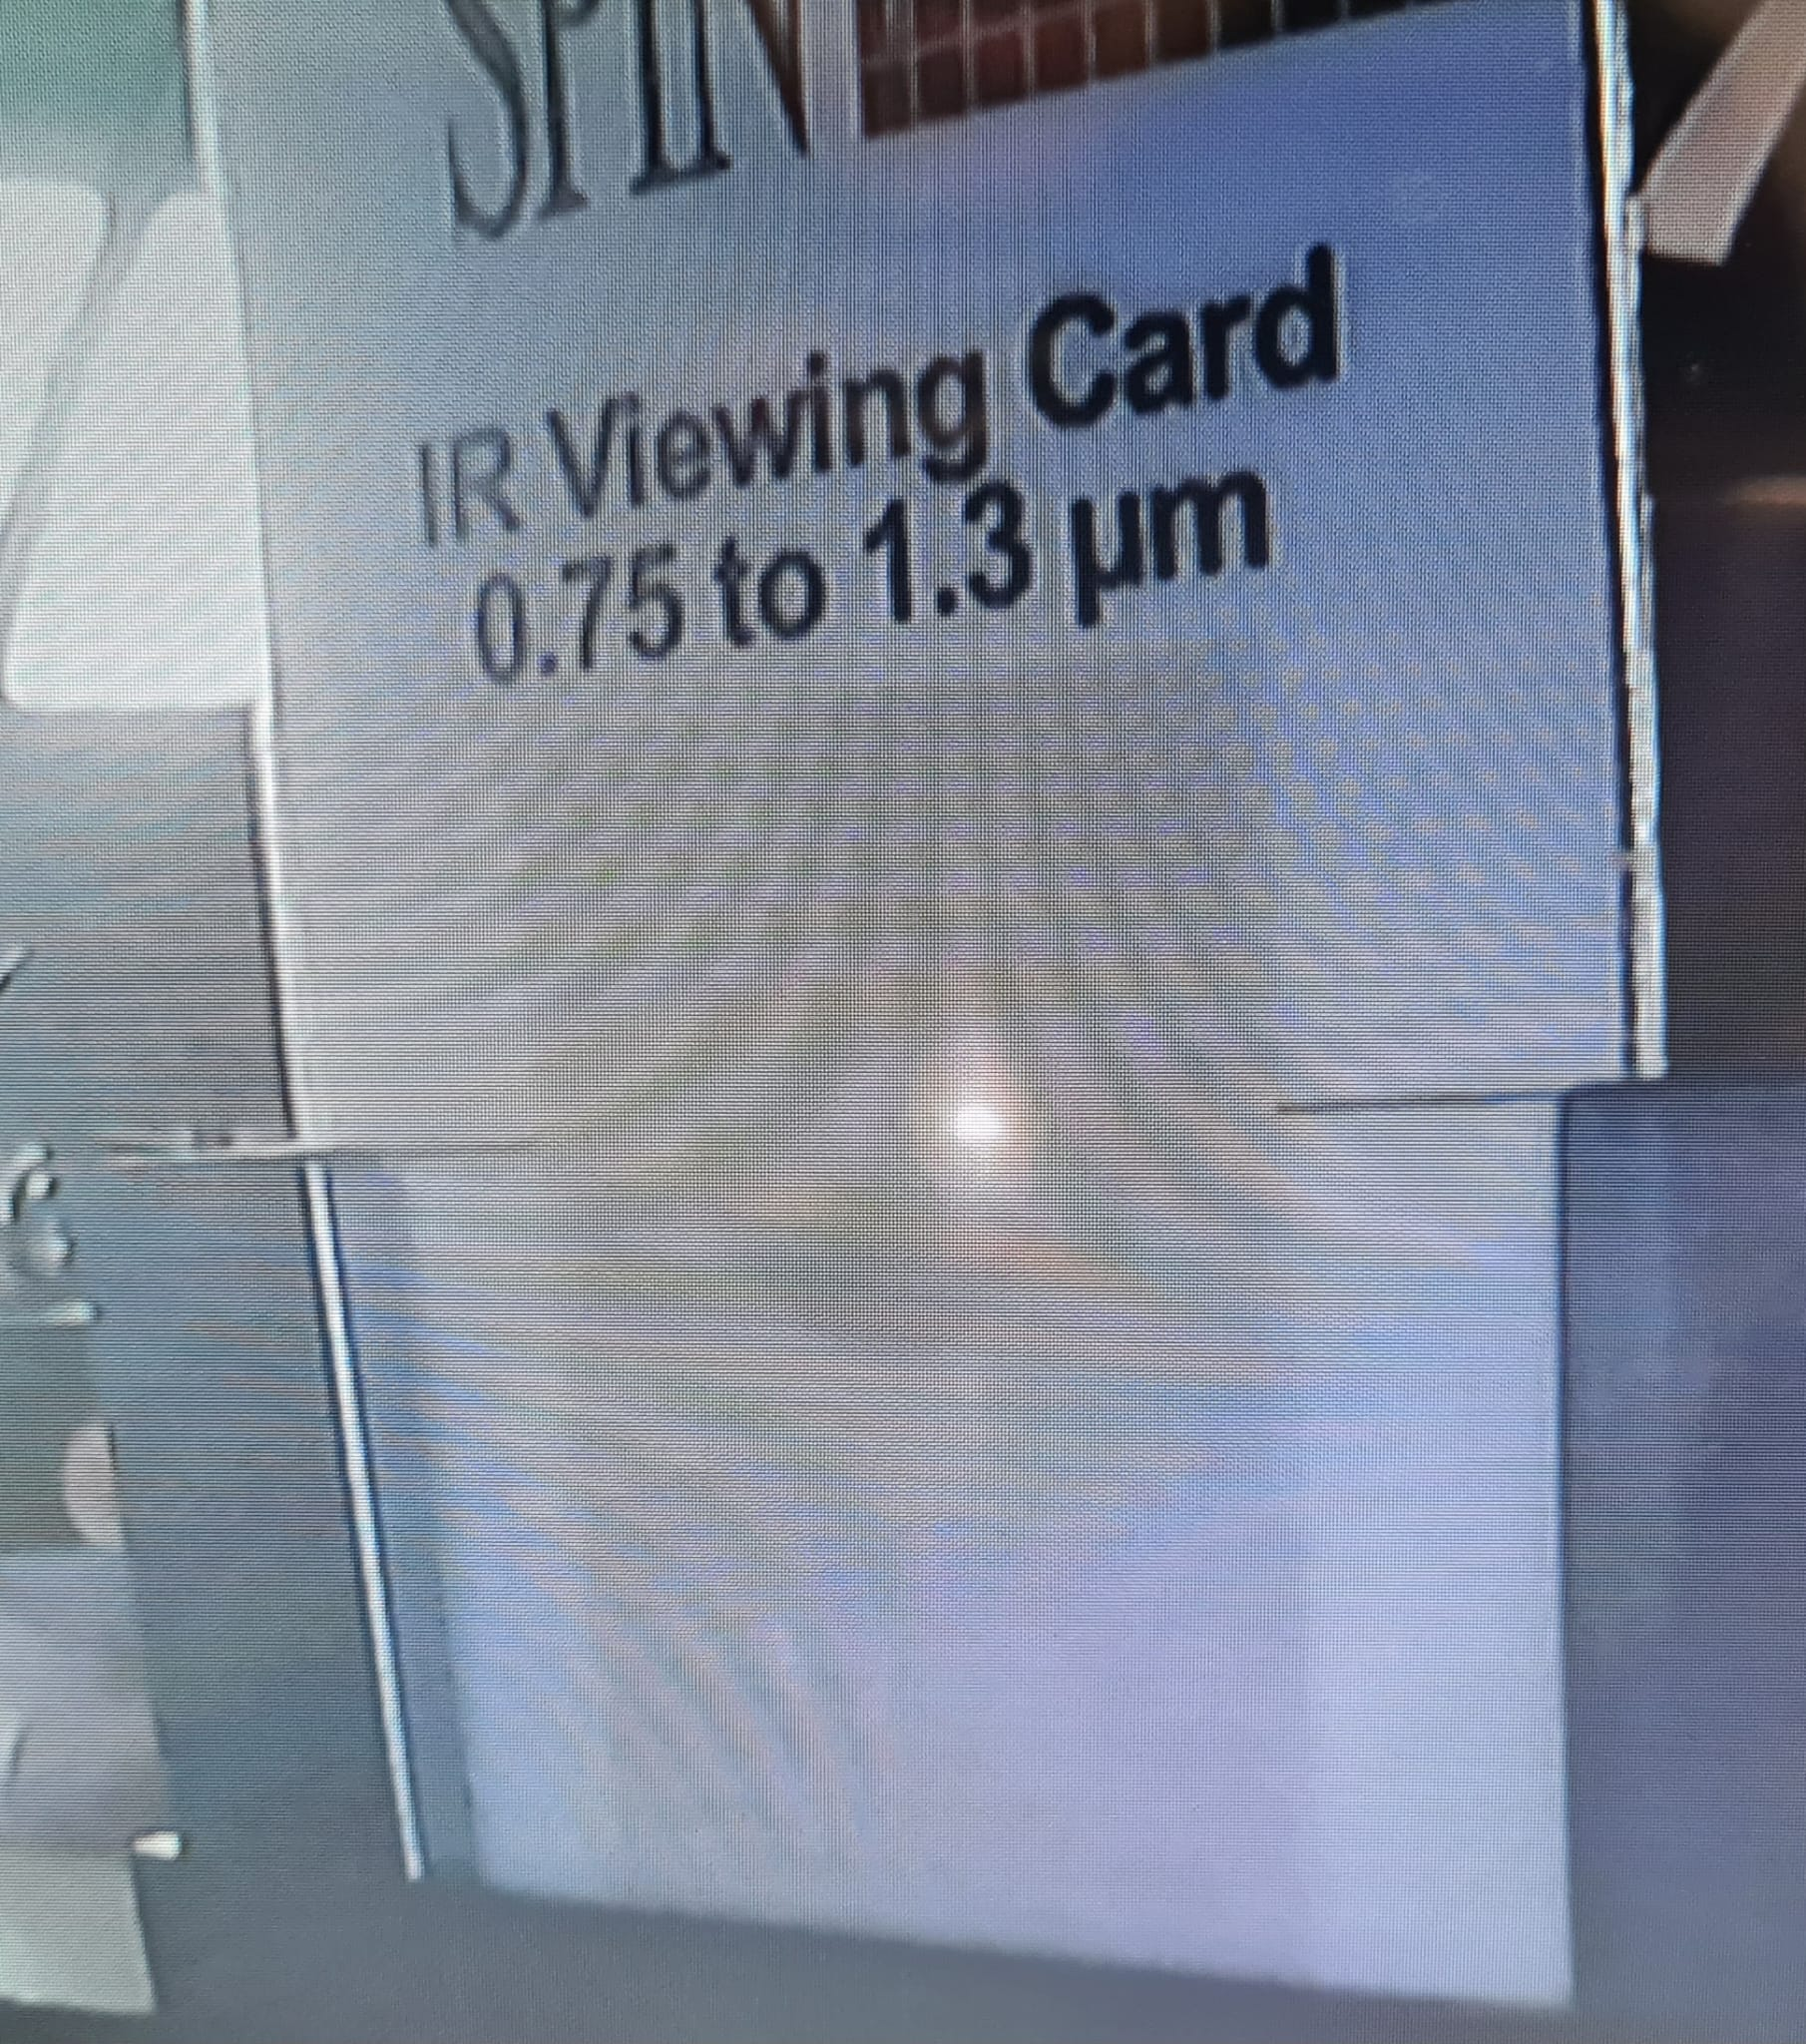
\includegraphics[width=0.6\textwidth]{content/pics/1.jpg}
        \subcaption{Strom unter Schwellenstrom.}
    \end{subfigure}
    \hfill
    \begin{subfigure}[c]{0.5\textwidth}
        \centering
        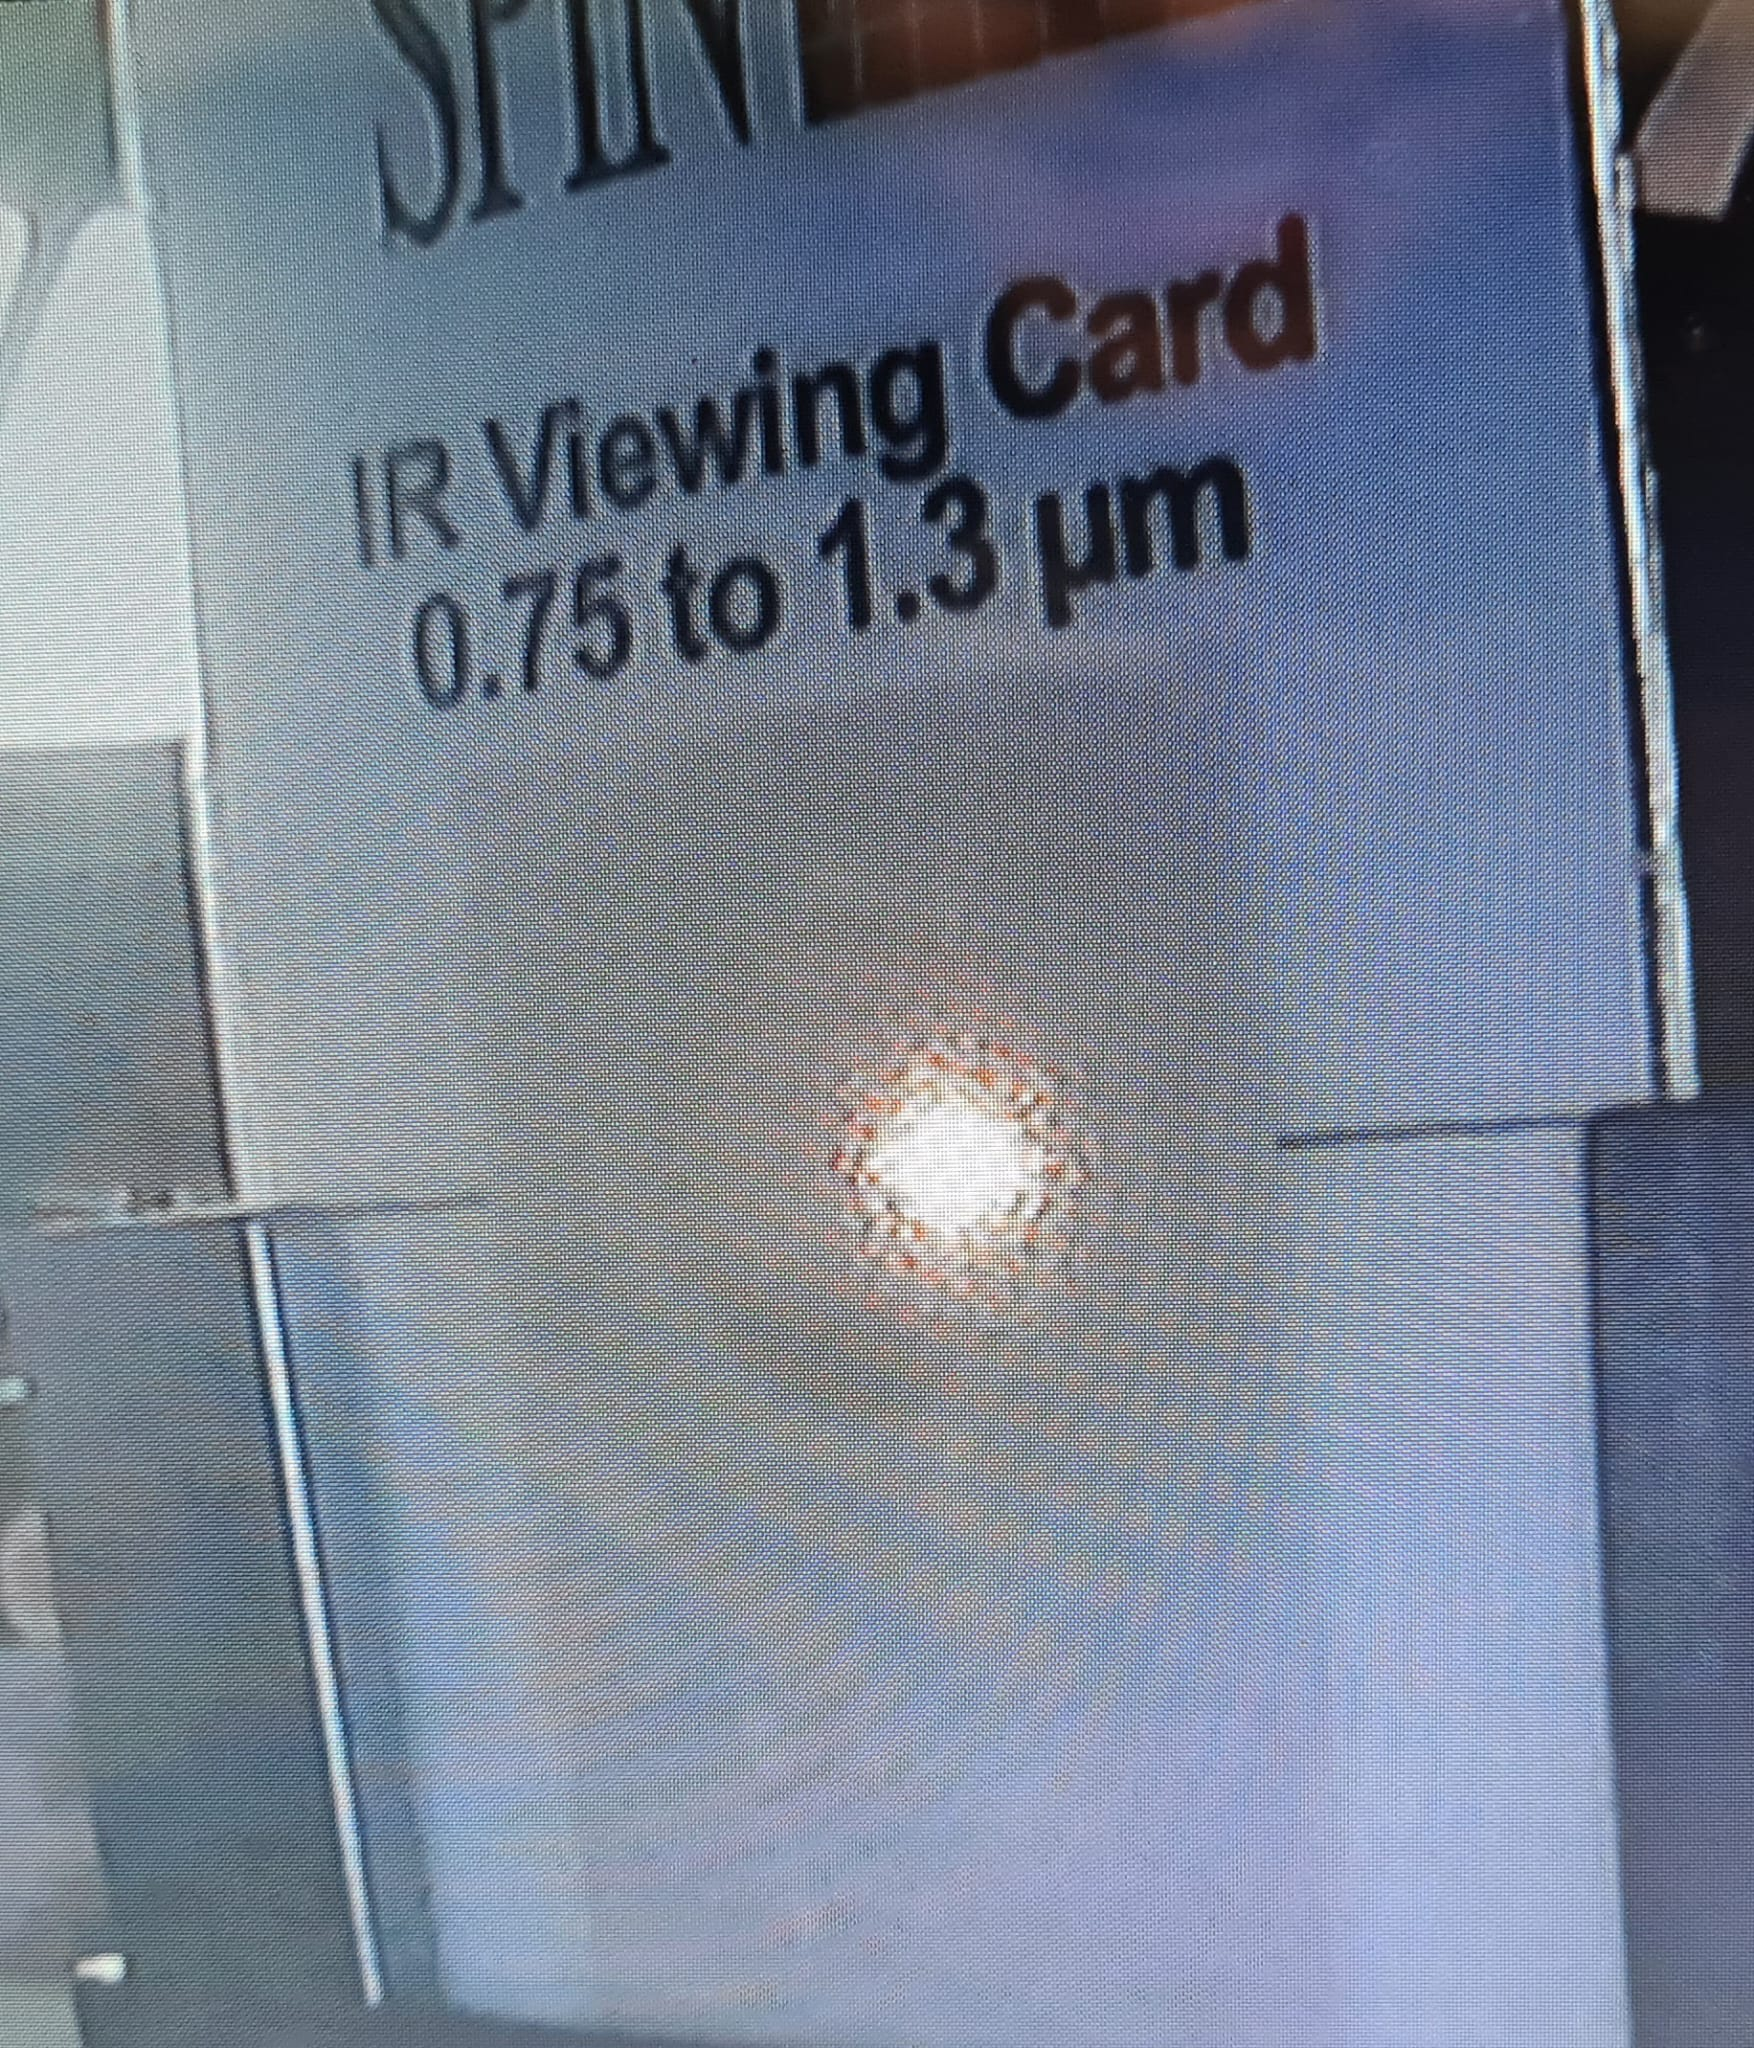
\includegraphics[width=0.6\textwidth]{content/pics/2.jpg}
        \subcaption{Strom genau gleich dem Schwellenstrom.}
    \end{subfigure}
    \hfill
    \begin{subfigure}[c]{0.5\textwidth}
        \centering
        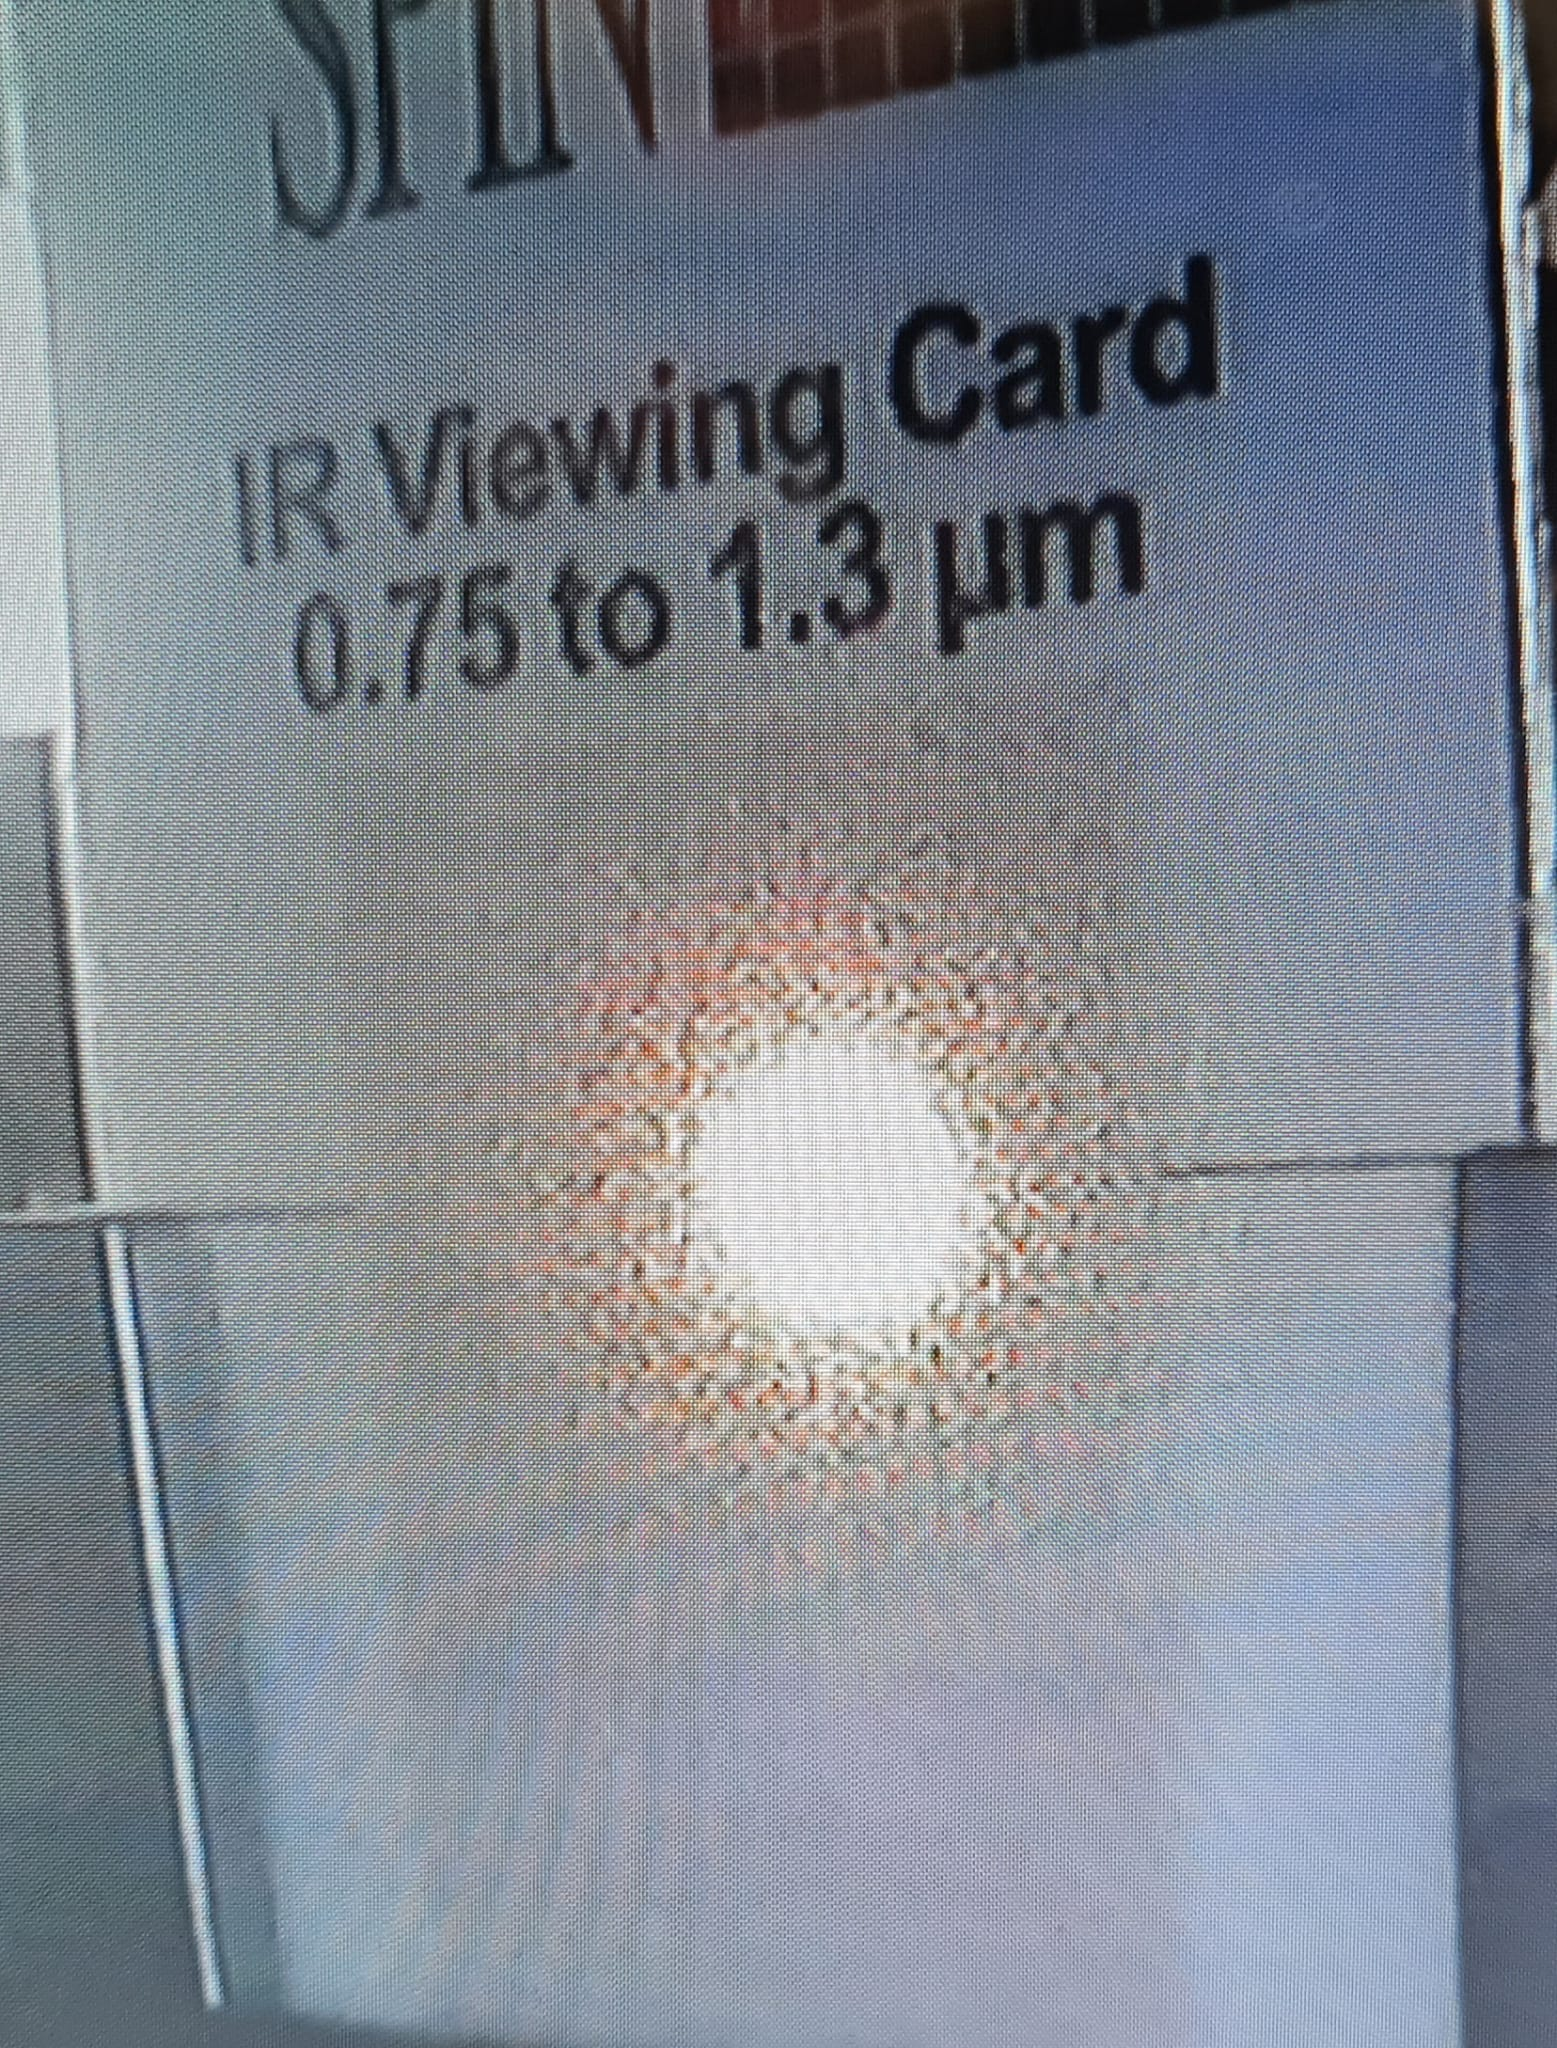
\includegraphics[width=0.6\textwidth]{content/pics/3.jpg}
        \subcaption{Strom über dem Schwellenstrom.}
    \end{subfigure}

    \caption{Bild der Detektorkarte mit und ohne Lasergranulation.}
    \label{fig:granulation}
\end{figure}

\subsection{Rubidiumfluoresenz}
\label{sec:rubidium}
Die Rubidiumfluoresenz kann nach erfolgreichem Einstellen der Apparatur beobachtet werden. Das aufgenommene Bild
dazu ist in \autoref{fig:lum} dargestellt.
\begin{figure}
    \centering
    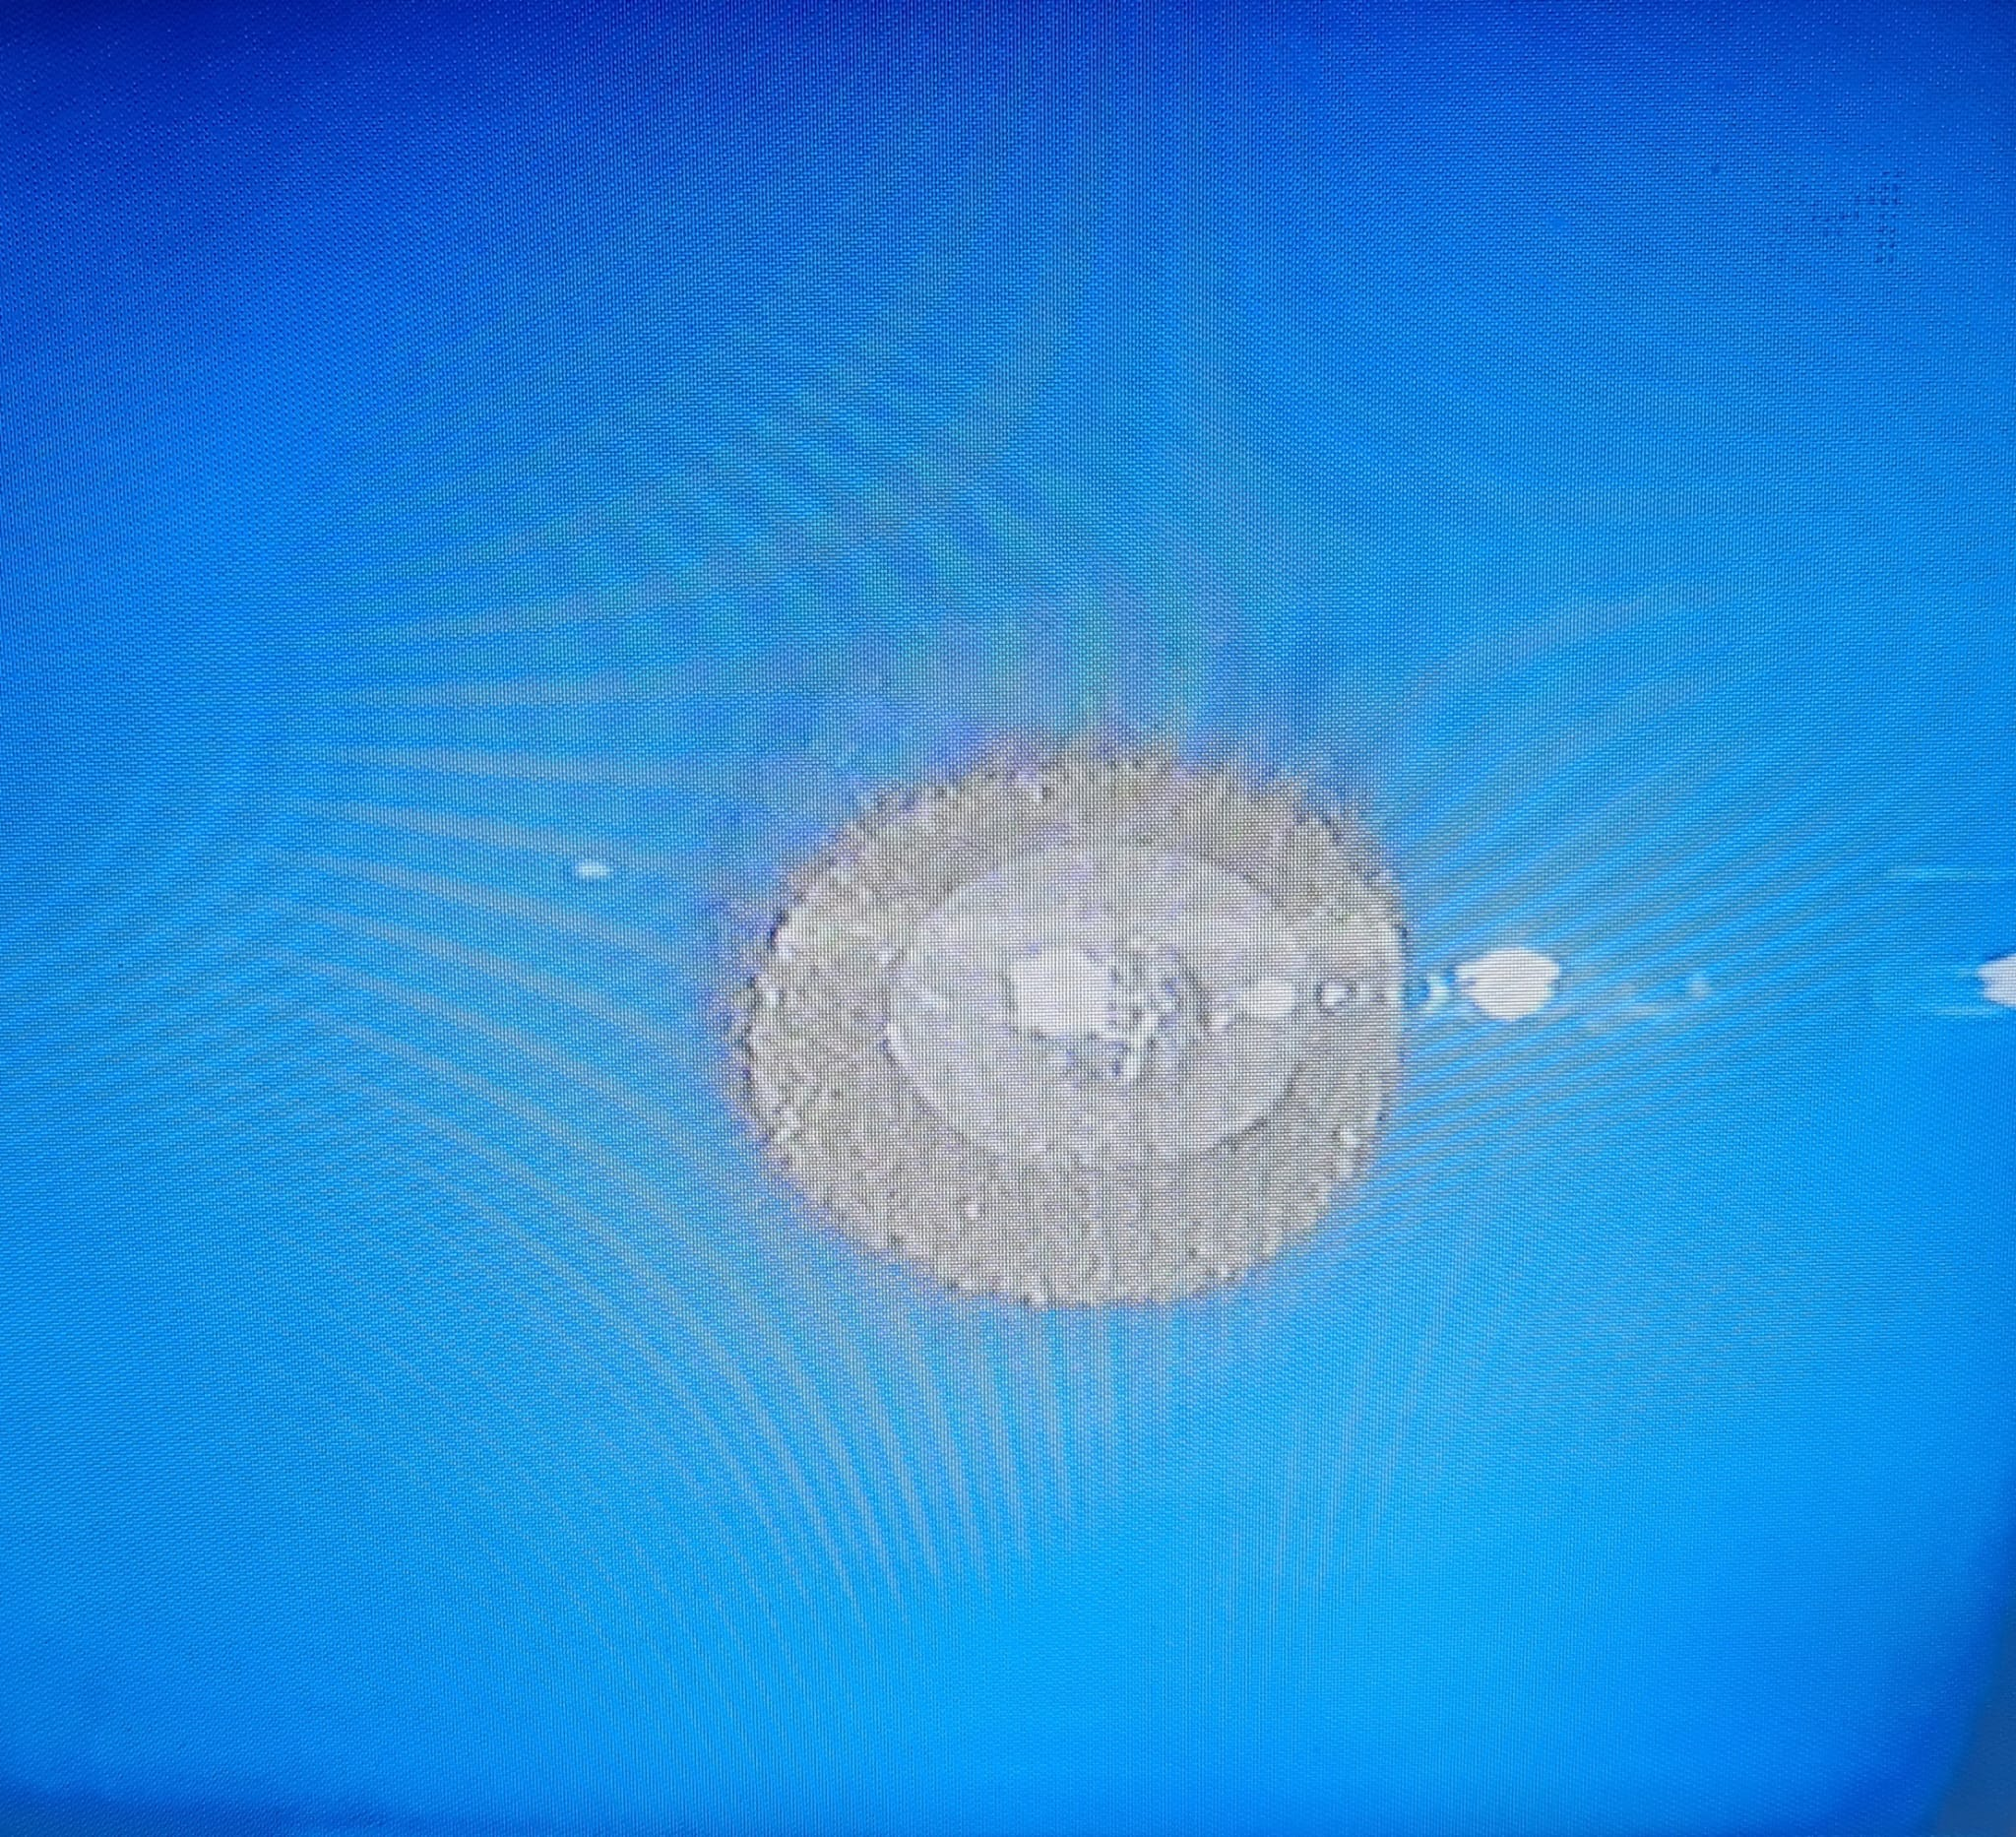
\includegraphics[height=6cm]{content/pics/4.jpg}
    \caption{Aufnahme der Rubidiumzelle bei Auftreten der Fluoresenz.}
    \label{fig:lum}
\end{figure}

\subsection{Transmissionsspektrum}
\label{sec:trans}
Das gemessene Transmissionsspektrum von Rubidium ist in \autoref{fig:trans} zu finden. Es lässt sich eindeutig
der in der Theorie vorhergesagtem Spektrum zu ordnen.
\begin{figure}
    \centering
    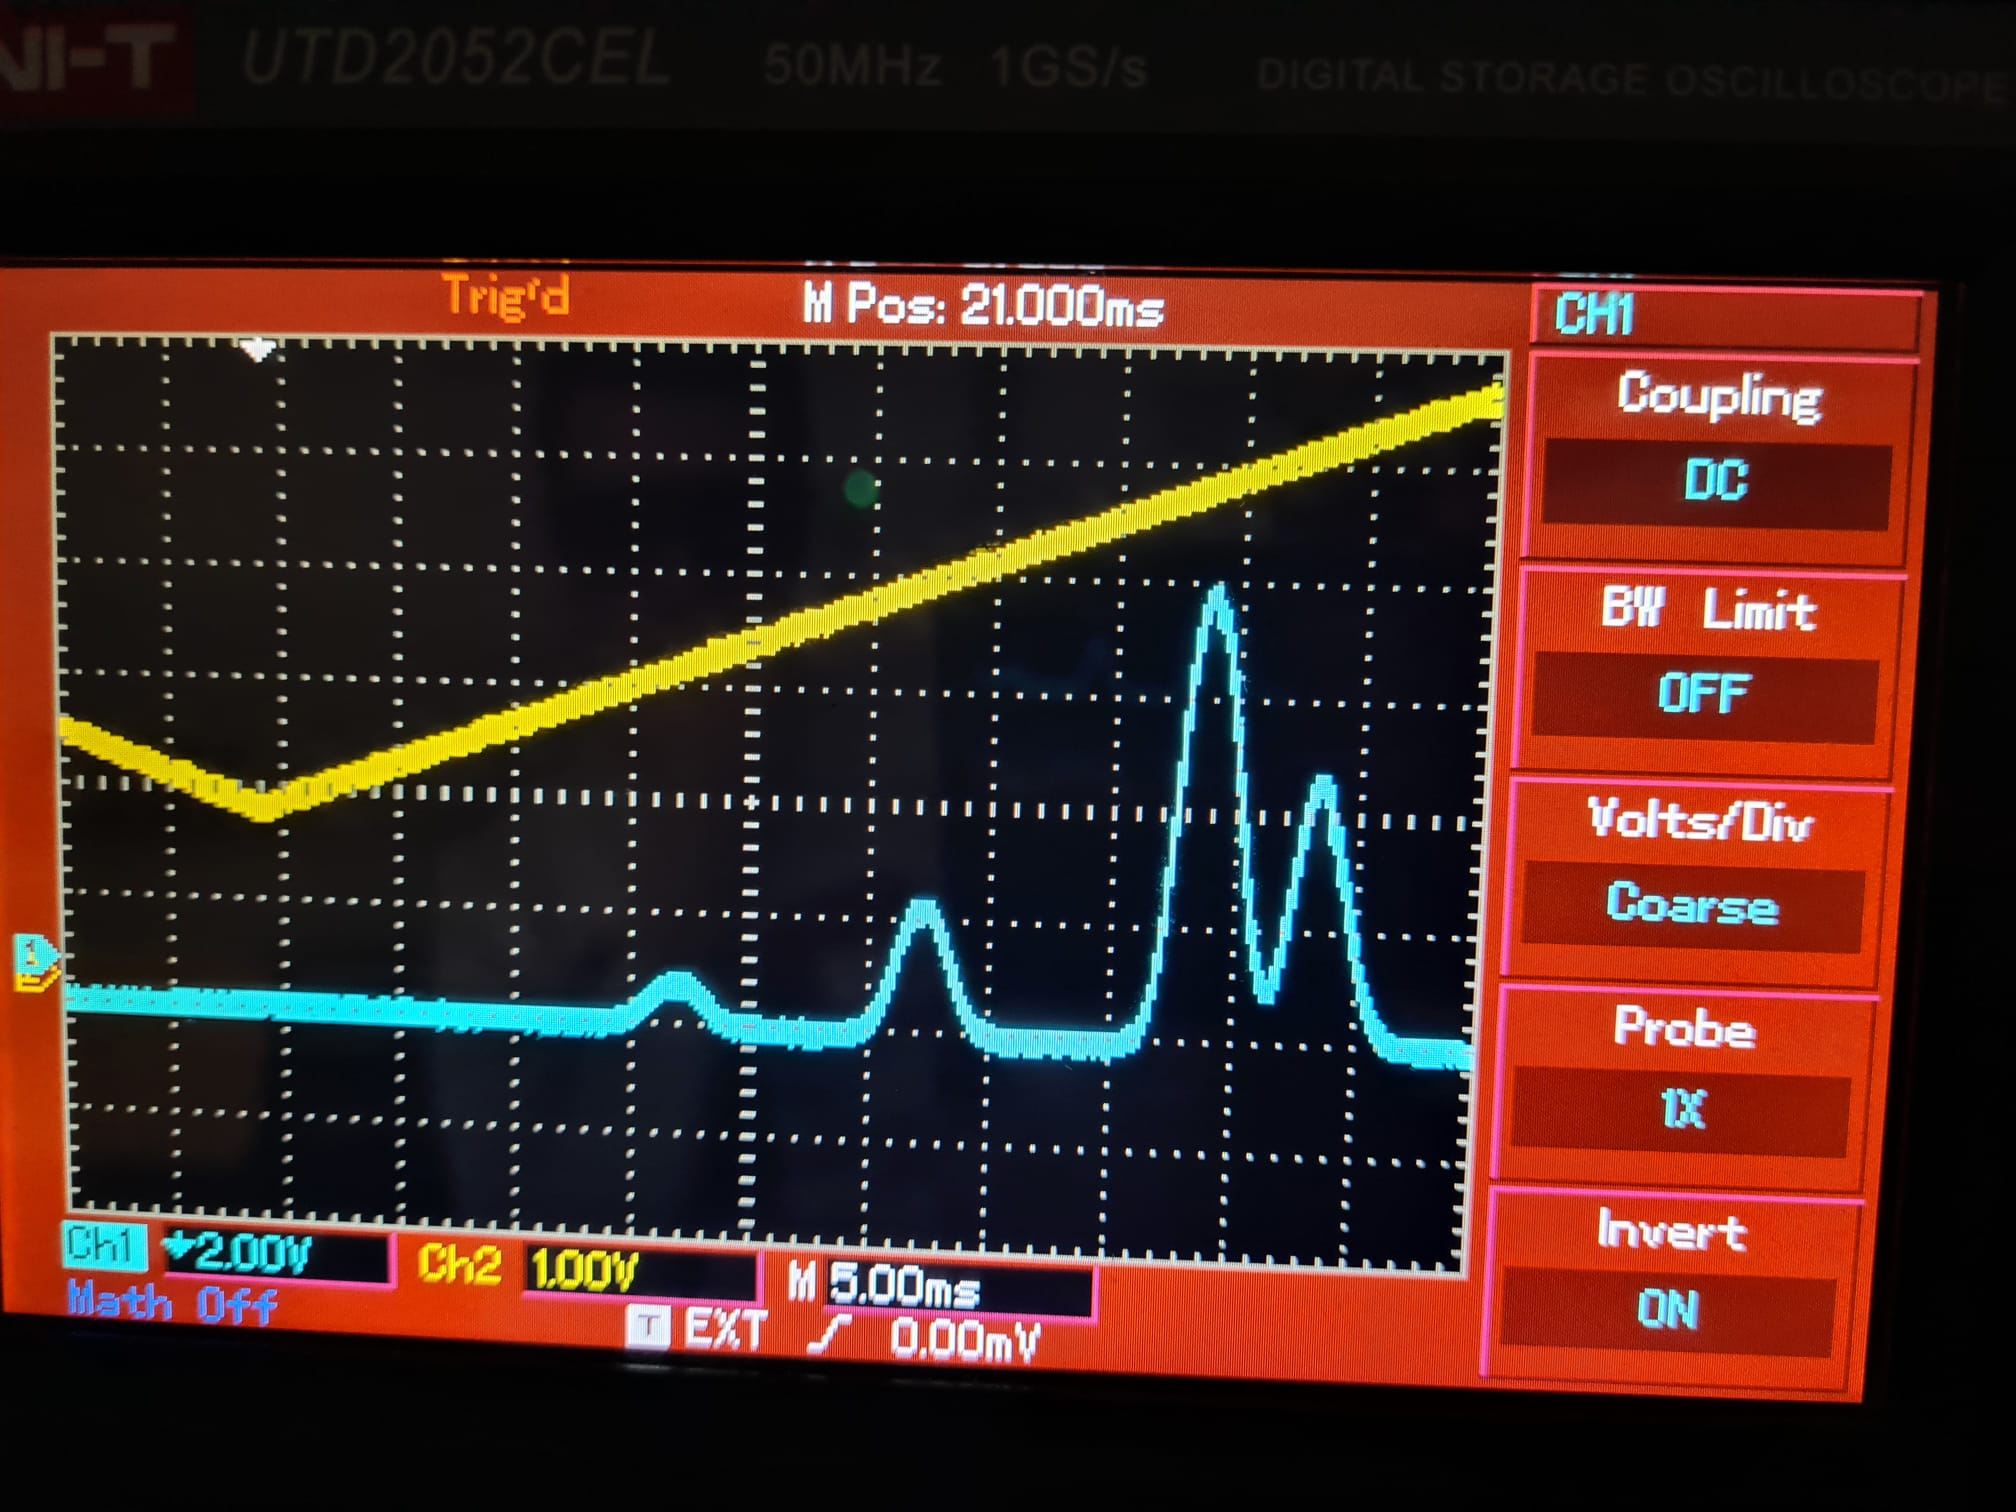
\includegraphics[height=6cm]{content/pics/5.jpg}
    \caption{Transmissionsspektrum von Rubidium.}
    \label{fig:trans}
\end{figure}